%----------------------------------------------------------------------------------------
% Plantilla LaTeX para Tesis o Tesina Posgrado FIC
% Autor: Esteban Hernandez Santiago
% Fecha de creación: 15/02/2024
% Descripción: 
%----------------------------------------------------------------------------------------

\documentclass{tFIC3} % Define la clase del documento

% Atributos de la tesis
\tituloTesis{Titulo de la Tesis o Tesina} % Establece el título de la tesis.
\nombreEstudiante{Nombre del Alumno} % Nombre del alumno autor de la tesis.
\setTipoDocumento{tesis} % Define el tipo de documento (tesis o tesina).
\nombrePrograma{MAESTRÍA EN CIENCIAS E INGENIERÍA DE DATOS} % Programa académico al que pertenece la tesis.
\anio{2024} % Año de publicación de la tesis.
\grado{1} % Nivel de grado (1 para Maestría, 2 para Especialidad).

\directorTesis{Nombre del Director} % Director de tesis.
\codirectorTesis{Nombre del Codirector} % Codirector de tesis, opcional.
\asesorUno{Nombre del Asesor 1} % Primer asesor de tesis.
\asesorDos{Nombre del Asesor 2} % Segundo asesor de tesis, opcional.
% \asesorTres{Nombre del Asesor 3} % Tercer asesor de tesis, opcional.
% \asesorCuatro{Nombre del Asesor 4} % cuarto asesor de tesis, opcional.
% \asesorCinco{Nombre del Asesor 5} % Quinto asesor de tesis, opcional.
\fechaLiberacion{15}{mayo}{2024} % Fecha de liberación de la tesis.

% Otros paquetes para algoritmos, ecuaciones, texto de relleno, y tablas mejoradas.
\usepackage{graphicx} % Paquete para incluir imágenes.
\usepackage{algorithm} % Para algoritmos
\usepackage{algpseudocode} % Para pseudocódigo en algoritmos
\usepackage{amsmath} % Para ecuaciones avanzadas
\usepackage{lipsum} % Para texto de relleno
\usepackage{booktabs} % Para tablas mejoradas

% Archivo de bibliografía
\addbibresource{referencias.bib} % Añade el archivo de bibliografía.

\begin{document}

% Elementos preliminares del documento (portada, contraportada, hoja de aprobación, etc.)
\portada
\contraportada
\hojaAprobacion

\agradecimientos % Opcional
\dedicatoria % Opcional

% Configuracion de numeración estilo romano
\pagenumbering{roman}
\setcounter{page}{1}

% Tablas de contenido
\contenido % Genera la tabla de contenidos.
\indiceFiguras % Lista de figuras.
\indiceCuadros % Lista de cuadros o tablas.
% Otros índices para ecuaciones, algoritmos, y apéndices.
\indiceEcuaciones % Opcional
\indiceAlgoritmos % Opcional
\indiceApendiceFiguras % Opcional
\indiceApendiceCuadros % Opcional

\resumen % Sección de resumen.
\summary % Sección de resumen en inglés.

% Configuracion de numeración estilo arábigo
\pagenumbering{arabic}
\setcounter{page}{1}

% CAPITULOS
\introduccion % I. INTRODUCCIÓN
\revisionLiteratura % II. REVISÍON DE LITERATURA
\materialesMetodos % III. MATERIALES Y MÉTODOS
\resultadosDiscusion % IV. RESULTADOS Y CONCLUSIÓN
\conclusiones % V. CONCLUSIONES
\bibliografia % VI. BIBLIOGRAFÍA

% APÉNDICES
\iniciarApendices % Comando para iniciar la sección de apéndices.

% Añadir un apéndice de figuras
% Comando para iniciar una nueva sección de apéndices
\apendice{APÉNDICE FIGURAS} % Inicia el apéndice de figuras con el título "APÉNDICE FIGURAS"

% A continuación, se incluyen ejemplos de cómo añadir figuras al apéndice.
% Estas figuras se añadirán a la lista de figuras de apéndices automáticamente.

% Ejemplo 1: Figura simple
\begin{appendixfigure}[htbp]
    \centering
    \includegraphics[width=0.75\linewidth]{example-image} % Ruta a la imagen
    \caption{Una descripción de la figura} % Título de la figura
    \label{fig:apendiceFigura} % Etiqueta para referencias cruzadas
\end{appendixfigure}

% Ejemplo 2: Figura con posición forzada (aquí)
\begin{appendixfigure}[H]
    \centering
    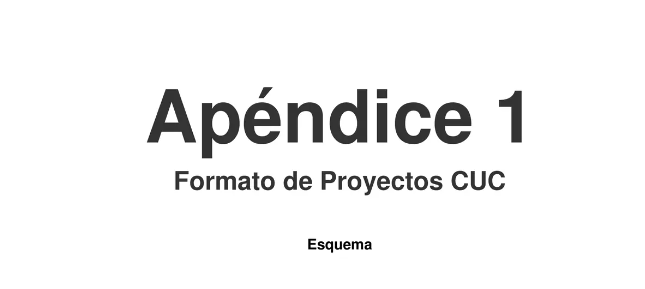
\includegraphics[width=0.75\linewidth]{Imagenes/image.png} % Ruta a la imagen
    \caption{\lipsum[1][1-2]} % Título de la figura con texto de ejemplo
    \label{fig:apendice} % Etiqueta para referencias cruzadas
\end{appendixfigure} % Opcional

% Añadir el apéndice de cuadros
% Comando para iniciar una nueva sección de apéndices
\apendice{APÉNDICE CUADROS} % Inicia el apéndice de cuadros con el título "APÉNDICE CUADROS"

% A continuación, se incluyen ejemplos de cómo añadir cuadros al apéndice.
% Estos cuadros se añadirán a la lista de cuadros de apéndices automáticamente.

% Ejemplo 1: Cuadro de datos básicos
\begin{appendixtable}[ht]
    \centering
    \caption{Ejemplo de un cuadro de datos básicos.} % Título del cuadro
    \begin{tabular}{ccr} % Estructura del cuadro: 3 columnas
        \toprule
        Columna A & Columna B & Columna C \\
        \midrule
        A1 & B1 & C1 \\
        A2 & B2 & C2 \\
        A3 & B3 & C3 \\
        \bottomrule
    \end{tabular}
    \label{tab:cuadro-datos-basico} % Etiqueta para referencias cruzadas
\end{appendixtable}

% Ejemplo 2: Cuadro de datos avanzados
\begin{appendixtable}[ht]
    \centering
    \caption{Ejemplo de un cuadro de datos avanzados.} % Título del cuadro
    \begin{tabular}{l|c|r} % Estructura del cuadro: 3 columnas con líneas verticales
        \toprule
        Columna 1 & Columna 2 & Columna 3 \\
        \midrule
        Dato 1 & Dato 2 & Dato 3 \\
        Dato 4 & Dato 5 & Dato 6 \\
        Dato 7 & Dato 8 & Dato 9 \\
        \bottomrule
    \end{tabular}
    \label{tab:cuadro-datos-avanzado} % Etiqueta para referencias cruzadas
\end{appendixtable}
 % Opcional

\end{document}